\documentclass[10pt,a4paper]{article}
\usepackage{amsmath}
\usepackage{amsfonts}
\usepackage{amssymb}
\usepackage[english]{babel}
\usepackage[left=2cm,right=2cm,top=2cm,bottom=2cm]{geometry}
\usepackage{graphicx}
\usepackage{hyperref} % Used for external links
\usepackage[utf8]{inputenc}
\usepackage{listings} % Used for source code listing

% Source code listing's parameters
\lstset{
  frame=single,
  keepspaces=true,
%  title=\lstname
}

\title{First Exercise\\{\small{Fundamentals Of Electronics - a.a. 2018-2019 -
University of Padua (Italy)}}}
\author{Pietro Prandini (mat. 1097752)}

\begin{document}
\maketitle
\section{Audio amplifier}
\subsection{Voltage gain and frequency domain - Ideal op. amp.}
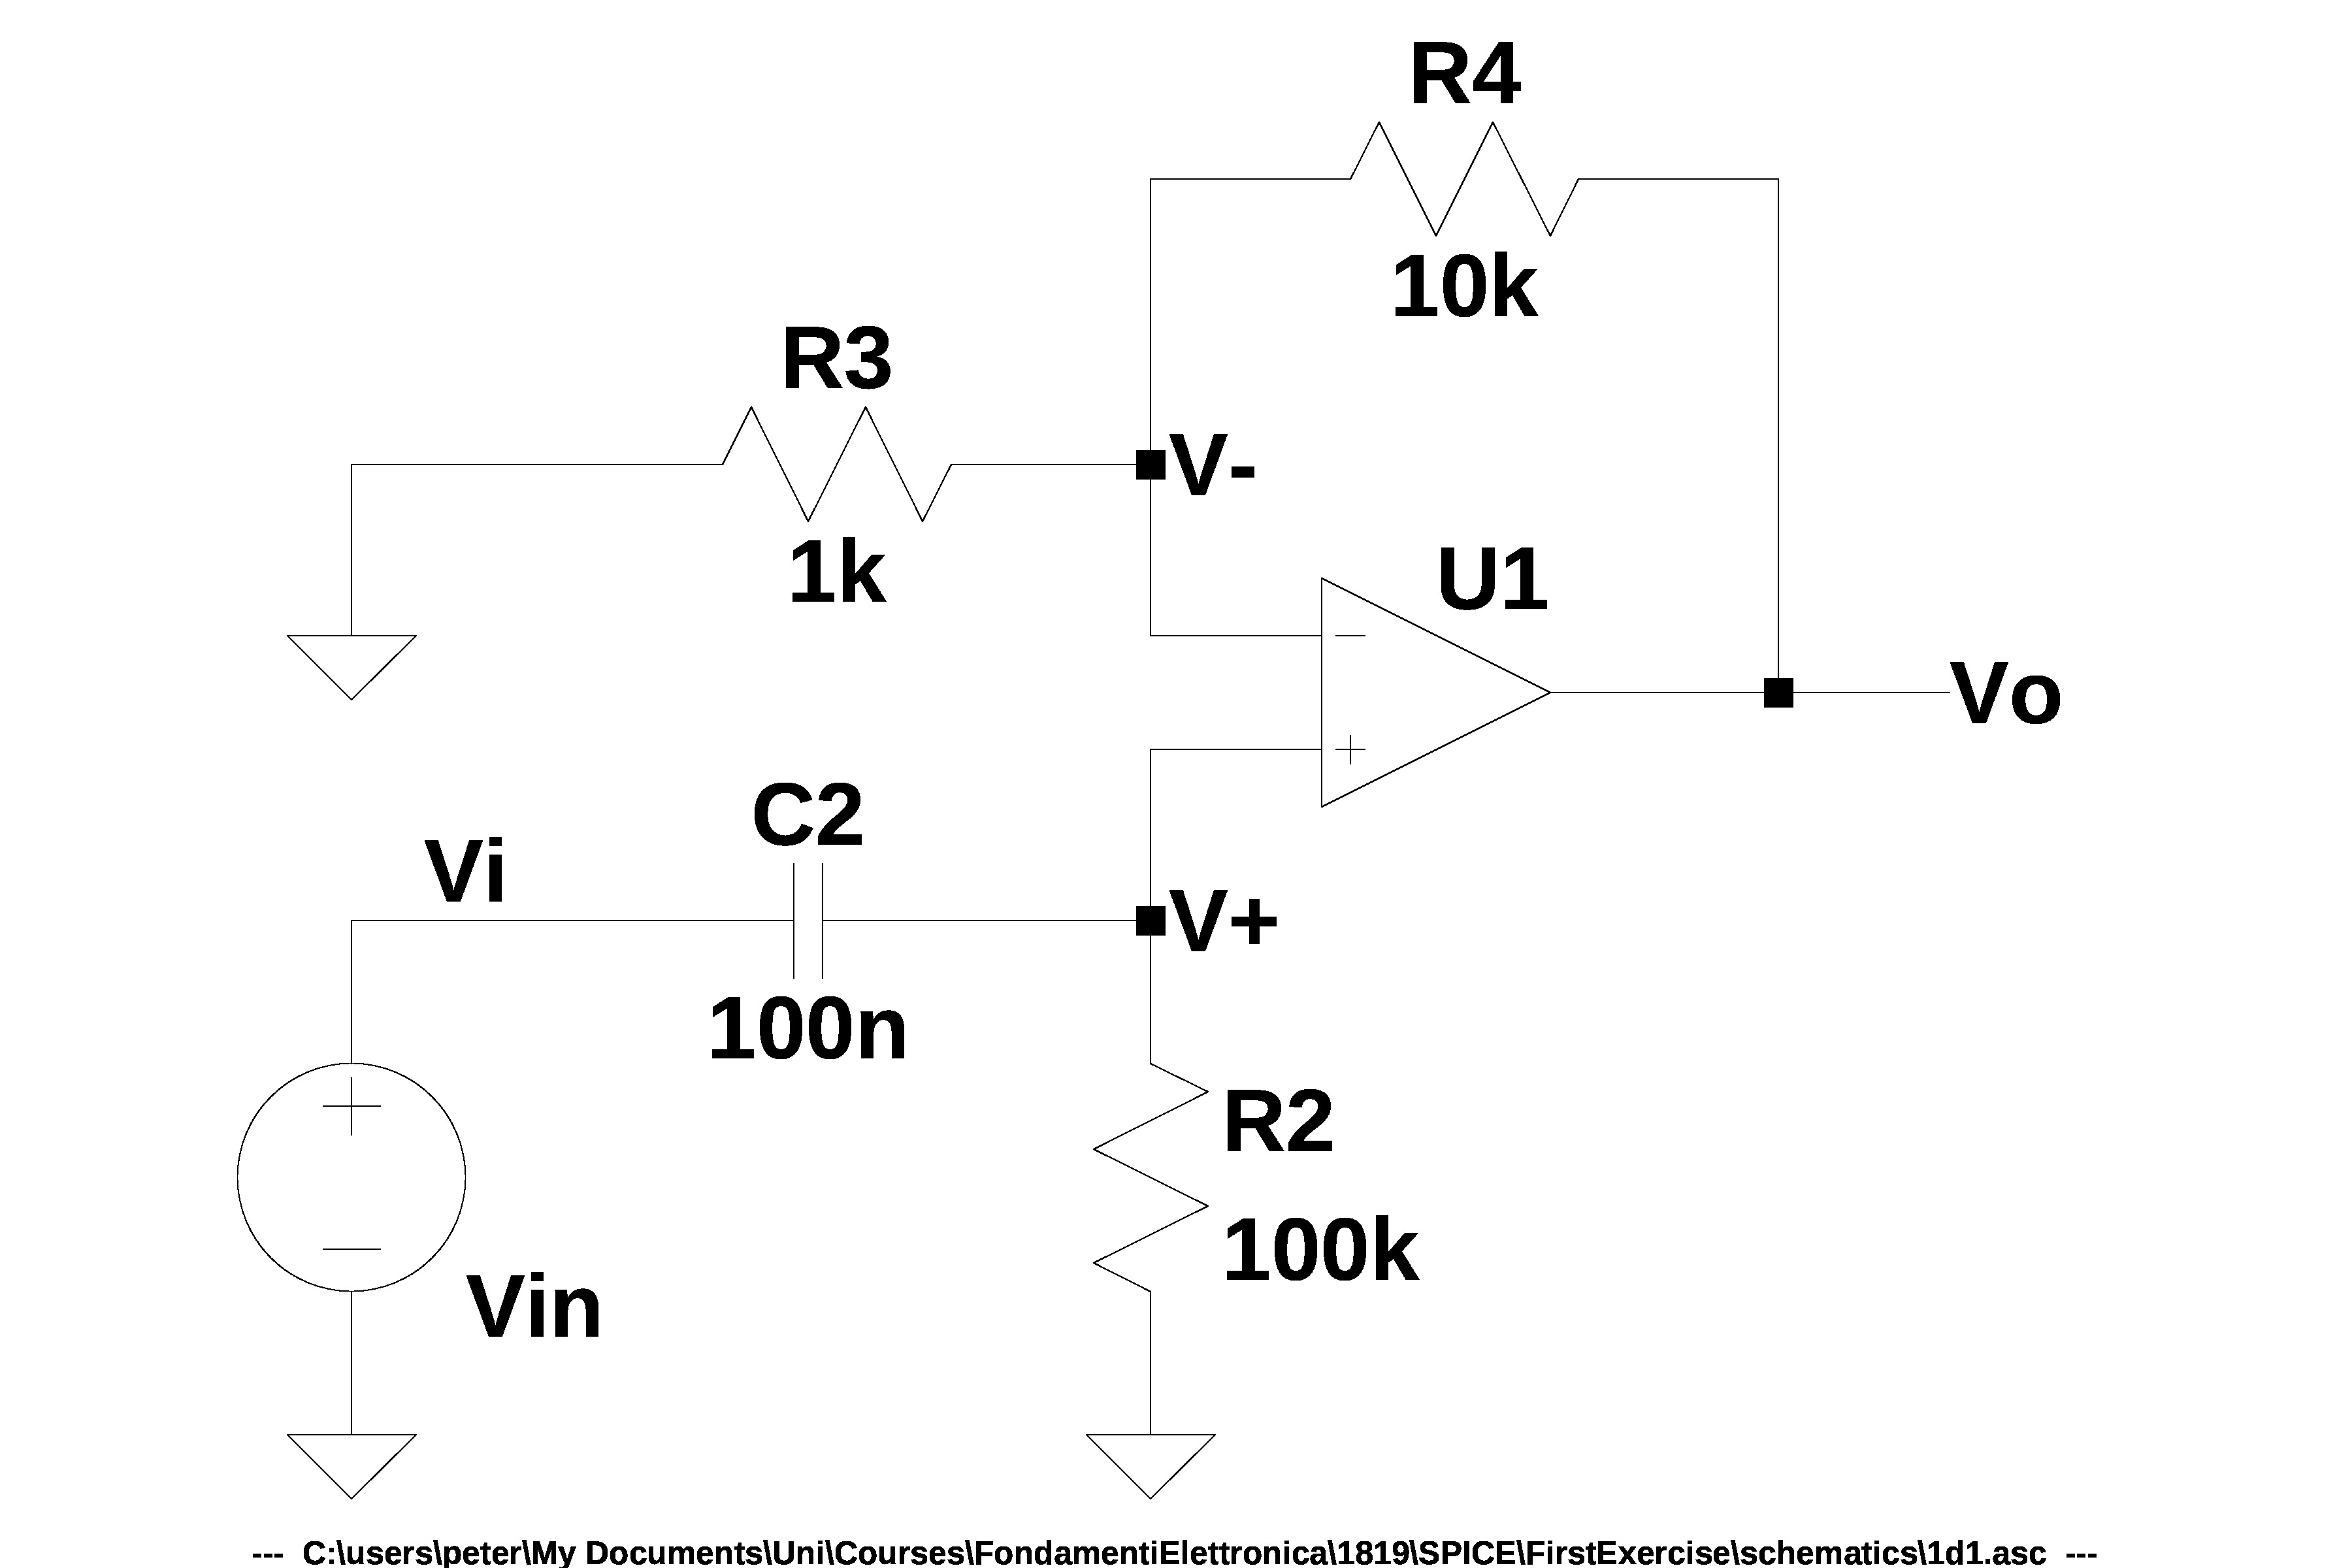
\includegraphics[width=8cm]{schematics/1d1.jpg}
\subsubsection{Netlist}
\lstinputlisting{netlist/1d1.cir}

%\subsubsection{Netlist}
%\lstinputlisting{netlist/PietroPrandini_FE_18-19_1.cir}

% License
\vspace*{\fill}
\centering
\tiny{This work is licensed under the Creative Commons Attribution-ShareAlike
 4.0 International License. To view a copy of this license, visit
 \href{http://creativecommons.org/licenses/by-sa/4.0/}{http://creativecommons.org/licenses/by-sa/4.0/}
or send a letter to Creative Commons, PO Box 1866, Mountain View, CA 94042,
USA.}

\end{document}
